
\subsubsection{ECal Trigger overview}


The proposed trigger system is nearly deadtimeless. The trigger decision goes to the Trigger Supervisor every 4 ns. The trigger supervisor can apply deadtime if necessary, for example on a 'busy' or 'full' condition from front-end electronics.


\begin{figure}[t]
\includegraphics[scale=0.5]{daq_trigger/figures/FADC250_Photo_001.jpg}
\caption{\small{Jefferson Lab FADC250 VXS module.}}
\label{fig:fadc}
\end{figure}

The information from top and bottom parts of the ECal will be sent to the Jefferson Lab FADCs (Flash Analog-to-Digital Converters), Fig.~\ref{fig:fadc},  located in two different VXS crates (see Fig.~\ref{fig:hps_trigger_cal}). FADC  works at the frequency 250~MHz; i.e. it measures the amplitude of each ECal channel every 4 ns. FADC has 12bit pulse digitizer for readout and trigger processing. 

The first stage components of the trigger logic are incorporated into the Flash ADC board's FPGAs, while the final decision is made in a Crate Trigger Processors (CTPs) and  Sub-System Processor (SSP) .
FADC sends the information about the pulse energy and time to CTP.


\begin{figure}[t]
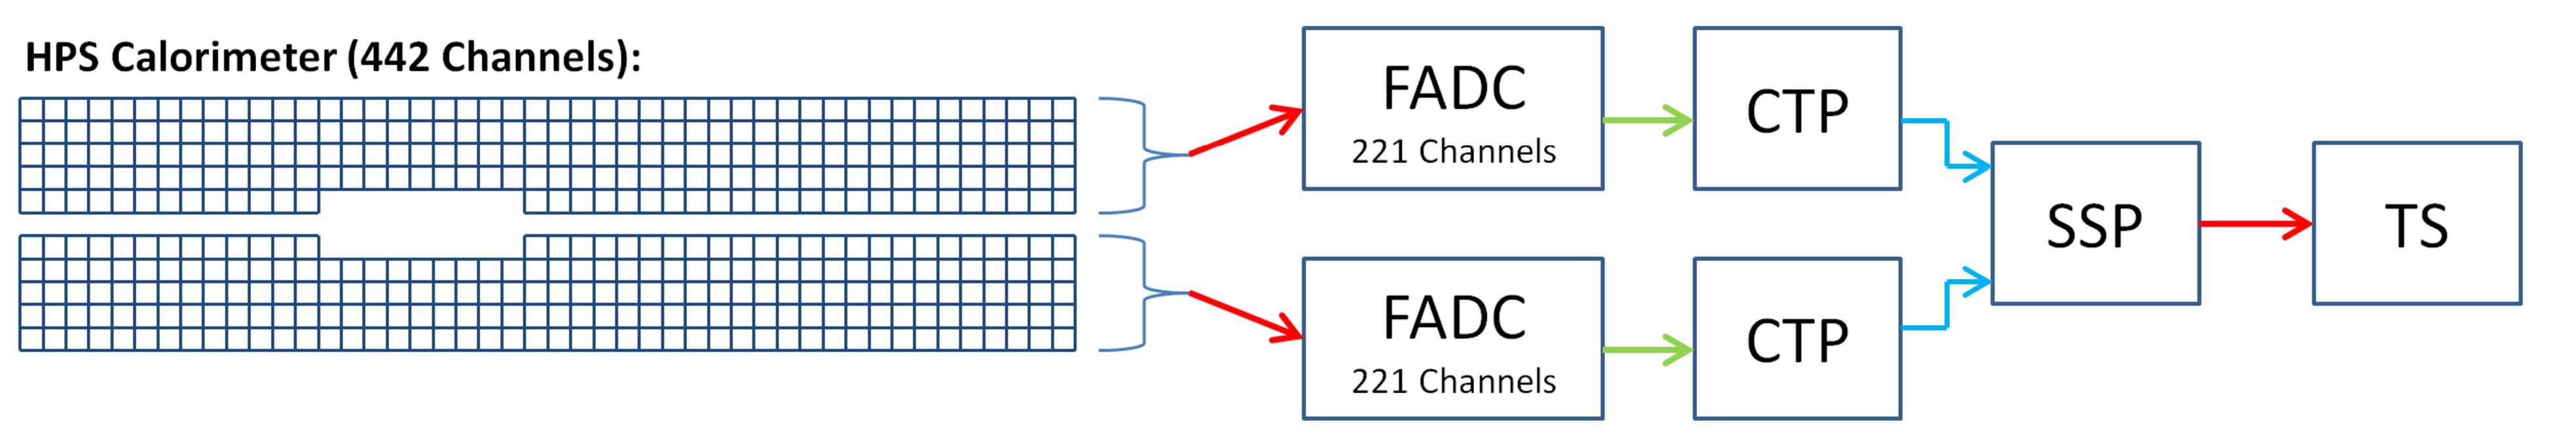
\includegraphics[scale=0.25]{daq_trigger/figures/hps_trigger_cal}
\caption{\small{ECAL trigger logic. FADC - Jlab Flash ADC, CTP - Crate Trigger Processor, SSP - Sub-System Processor, TS - Trigger Superviser.}}
\label{fig:hps_trigger_cal}
\end{figure}

The trigger system can be broken down into the following 3 sections:
 \begin{itemize}
 \item FADC (pulse finding): Samples the detector channel to find pulses. Pulse energy and times are sent to CTP.
 \item CTP (cluster finding): Searches FADC pulses (from half of calorimeter) to find clusters. Cluster energy, time, and hit pattern sent to SSP.
 \item SSP (cluster pair finding): Searches CTP clusters (from top and bottom) to find cluster pairs and create the trigger. Trigger cuts on pairs decide final trigger.
 \end{itemize}
 
 Trigger logic will search for a time coincidence between two clusters in opposite halves of ECal that occur within a programmable time window with 4ns resolution. The maximum trigger decision time (latency) is currently set to 3 $\mu$s for Level 1. That value is defined by the SVT readout APV25 chip.

The Trigger Supervisor generates all necessary signals, and controls the entire DAQ system readout through the Trigger Interface units. The Trigger Interface (TI) units installed in every crate participate in the readout process. The system is free-running and driven by a 250MHz global clock. The maximum trigger accept rate is 50 KHz.

%\subsubsection{Jefferson Lab FADC}

\subsubsection{Jefferson Lab FADC}

The main characteristics of the Jefferson Lab Flash ADC are as follows:
\begin{itemize}
\item 12 bits digitizer with 250Msps
\item 50$\Omega$ termination input
\item Front-end input range  -0.5V, -1V or -2V.  Input range has to be above maximum pulse height to ensure no signal clipping
\end{itemize}

The FADC charge resolution as a function of the front-end input range is presented in Table~\ref{tab:charge_resolution}.
\begin{table}[h]
\centering
\begin{tabular}{| l | l |}
\hline
Input Range & Nominal Charge Resolution\\\hline
-0.5V & \ 9.76 fc per ADC count \\\hline
-1.0V & 19.53 fc per ADC count \\\hline
-2.0V & 39.06 fc per ADC count \\\hline
\end{tabular}
\caption{FADC charge resolution for different front-end input ranges.}
\label{tab:charge_resolution}
\end{table}

FADC data paths for the readout and trigger operation  are presented in Fig.~\ref{fig:hps_trigger_data}.
There are two FADC operation modes: the readout mode and trigger mode.

 In readout mode FADC determines the energy of the one ECal channel that will be reported. 
The channel integration occurs only if the input signal crosses the programmable threshold level.  Then a programmable number of samples around the threshold crossing are added together to form the reported integral.  The readout  mode has the following parameters for every FADC channel (see Fig.~\ref{fig:hps_trigger_data}, top panel):
 \begin{itemize}
 \item Number of samples integrated before the threshold crossing (NSB)
 \item Number of samples integrated after the  threshold crossing (NSA)
 \item Readout threshold, measured in ADC counts.
 \end{itemize}
 
The number of samples for a given channel integration  is the sum of NSB+NSA samples that will be stored in  
 the 17-bit FADC register. It is a fixed gate width pulse integration and there is no pedestal subtraction in the sum (pedestal subtraction happens offline).
 

 

\begin{figure}[t]
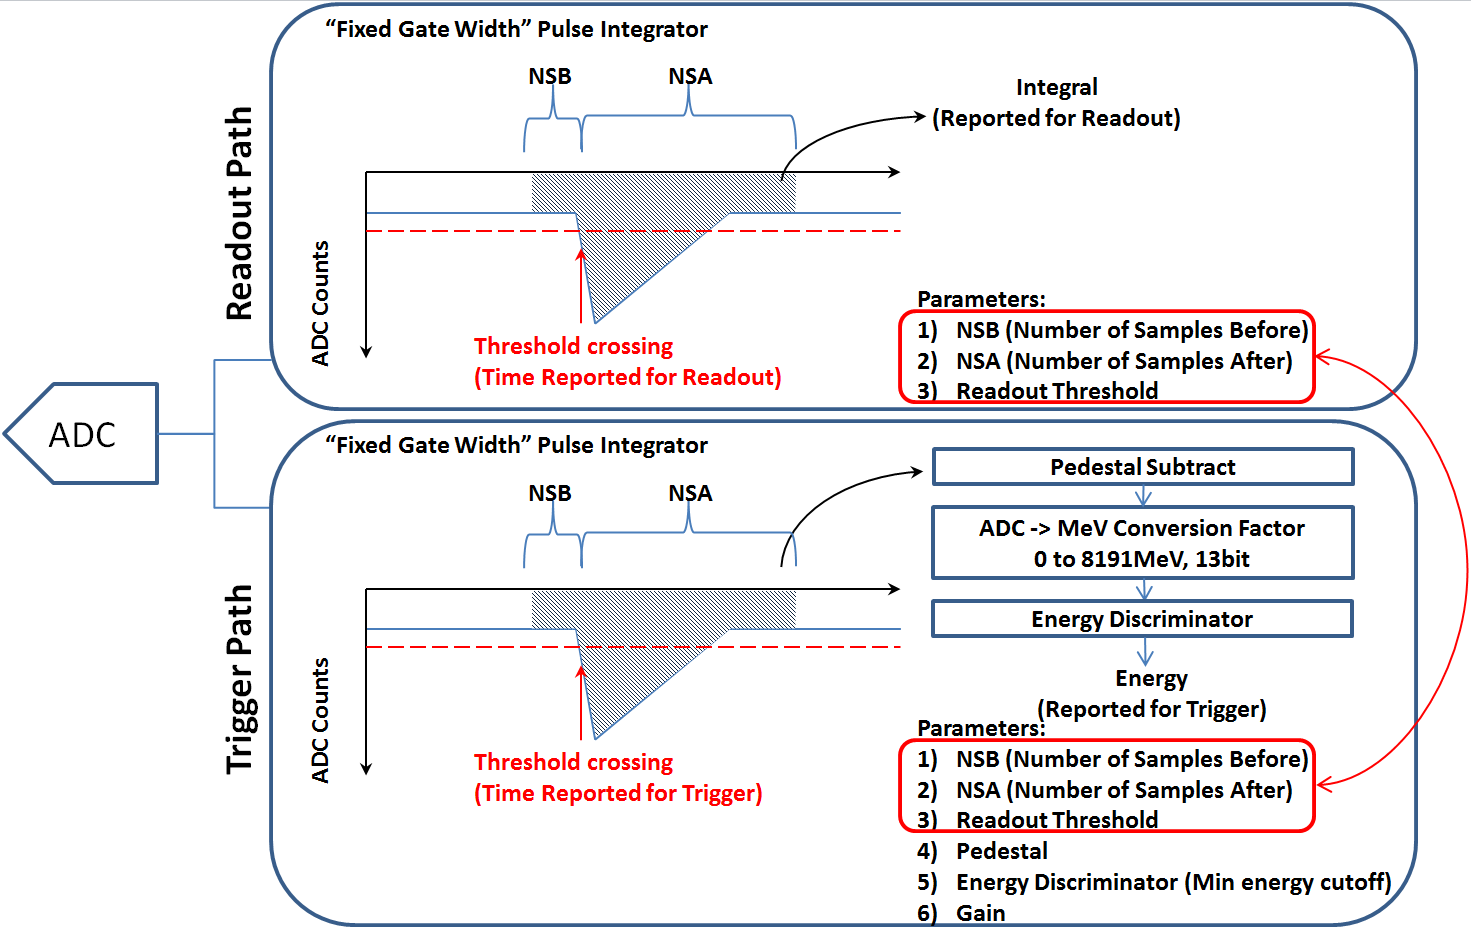
\includegraphics[scale=0.4]{daq_trigger/figures/hps_trigger_data}
\caption{\small{FADC data paths}}
\label{fig:hps_trigger_data}
\end{figure}

A block diagram of the HPS  trigger processing is shown in Fig.~\ref{fig:hps_trigger_data}, bottom panel. 
The trigger processing mode has the following parameters for every FADC channel:
 \begin{itemize}
 \item Number of samples integrated before the threshold crossing (NSB)
 \item Number of samples integrated after the  threshold crossing (NSA)
 \item Readout threshold, measured in ADC counts.
 \item Pedestal
 \item Conversion factor (gain) that converts  ADC channel to MeV, from 0 to 8191 MeV, 13 bits
 \item Energy discriminator (minimum energy cutoff)
 \end{itemize}
The parameters NSB, NSA and readout threshold are the same as in the readout mode.
The pedestal value is then subtracted from the integrated sum over NSB+NSA samples and this value is converted to MeV units using the gain conversion factor. The energy can be discriminated to cut off low energy pulses before reporting to the CTP. The value reported to the CTP is a 13bit pulse energy with a 4ns timing resolution where it crossed the readout threshold. Pulse data for every channel is sent to the CTP every 32ns (if there is no hit a 0 energy pulse is sent still). This sets a worst case double pulse resolution of 32ns per channel, but it can be as less than this if pulses occur in different 32ns windows, but close together).



%\subsubsection{Crate Trigger Processor} 

\subsubsection{Crate Trigger Processor} 

The Crate Trigger Processor receives the energy pulses (in MeV) and time stamp from each FADC channel in the crate (see Fig.~\ref{fig:hps_trigger_3x3}).
The algorithm used for cluster finding makes use the parallel processing nature of FPGAs by simultaneously searching for 125 clusters up to 3x3 in size across the calorimeter crystal array.  
A Cluster Processor (CP) algorithm:

\begin{itemize}
\item Add energy from hits together for every 3x3 square of channels in ECal
\item Hits are added together if they occur (leading edge) within a programmable number of clock cycles of each other (4 ns steps)
\item If 3x3 energy sum $\ge$  the programmable cluster energy threshold CTP reports cluster to the Sub-System processor the cluster parameters (time, energy, position and 3x3 hit pattern. 
\end{itemize}

Every 4ns the CTP evaluates all hits in its half of the calorimeter. A programmable time window is used to allow hits that are out of time with each other be considered as part of a cluster sum. This is done by reporting hits when they occur and then reporting them again for the next N number of 4 ns clock period, where N can be 0 to 7. This is useful to deal with skew and jitter that develop from the detector, cabling, and electronics.

When the sum of all hits in the 3x3 window occurring in a programmable time window are greater than the programmable energy threshold the cluster processor will report this cluster to the SSP if the energy is greater than all neighboring (up, down, left, right, and diagonals) 3x3 window cluster energies for that clock cycle. If the energy is not greater than its neighbor it will not be reported, but the neighbor will report if it is the greatest. The reason for this filtering is because there are several 3x3 windows that overlap and see the sample crystals and also many physics single clusters are larger than a 3x3 window.

The reported clusters to the SSP contain:

\begin{itemize}
\item 13bit Cluster energy (MeV)
\item Cluster position (crystal index: x,y)
\item Cluster time (4ns resolution)
\item Cluster hit pattern 3x3 (detector channels reporting a hit in the cluster)
\end{itemize}

The cluster position is the coordinate of the cluster processor that reported the cluster, which is where the peak cluster energy was seen from a 3x3 view. The 3x3 cluster hit pattern can be used by the SSP to help filter strange cluster patterns and/or make a low resolution cluster centroid computation.

\begin{figure}[h]

\includegraphics[scale=0.4]{daq_trigger/figures/hps_trigger_3x3}
\caption{\small{Cluster finding algorithm.}}
\label{fig:hps_trigger_3x3}
\end{figure}

%\subsubsection{Sub-System Processor} 

\subsubsection{Sub-System Processor} 

The cluster's time, energy, position and 3x3 pattern found in two VXS crates are reported to the Sub-System Processor. 
The SSP collects the cluster information from the full calorimeter and can create the trigger decisions of two types:
single cluster trigger and multi-cluster triggers.
Single cluster trigger condition includes the check on the cluster energy, $E_{min}\le E_{cluster}\le E_{max}$, where $E_{min}$ and $E_{max}$ are programmable minimum and maximum cluster energy.

Pairs trigger includes more conditions
\begin{itemize}
\item Energy sum,  
$E_{min}\le E_{top}+E_{bottom}\le E_{max}$
\item Pair time coincidence, 
$|t_{top}-t_{bottom}|\le \Delta t_{max}$ 
\item Energy difference, 
$|E_{top}-E_{bottom}|\le \Delta E_{max}$ 
\item Energy slope,
$E_{cluster\_with\_min\_energy}+R_{cluster\_with\_min\_energy}\times F_{energy}\le Threshold_{slope}$
\item Co-planarity, 
$|
tan^{-1}(\frac{X_{top}}{Y_{top}})-
tan^{-1}(\frac{X_{bottom}}{Y_{bottom}}) |\le Coplanarity_{angle}$
\item Number of hits in 3x3 window, 
\#$hits_{3\times 3}\ge HitThreshold$
\end{itemize}
\noindent
where $ E_{max}$,  $\Delta t_{max}$, $ \Delta E_{max}$ , $Threshold_{slope}$, 
$F_{energy}$, $Coplanarity_{angle}$
and
$HitThreshold$ are programable parameters.


Online event analysis will be provided to be compared against trigger event data for immediate verification (on each trigger cut: cluster energies, positions, timing, energy slope, coplanarity and hit threshold). With identical ADC readout and trigger pulse processing and high energy resolution, very precise agreement can be expected between trigger and readout.

%\subsubsection{Diagnostic Tools}

\subsubsection{Diagnostic Tools}

The previous experience with the similar (but much more simpler) trigger system showed that diagnostic tools are necessary to make sure that the calorimeter and trigger electronics work as expected. 

Scalers will be implemented for every ECal channel. The example of this diagnostic tool is presented in Fig.~\ref{fig:dvcs_beam}
from the previous version of the calorimeter. Hot or dead channels are easily identified online.
\begin{figure}[h]
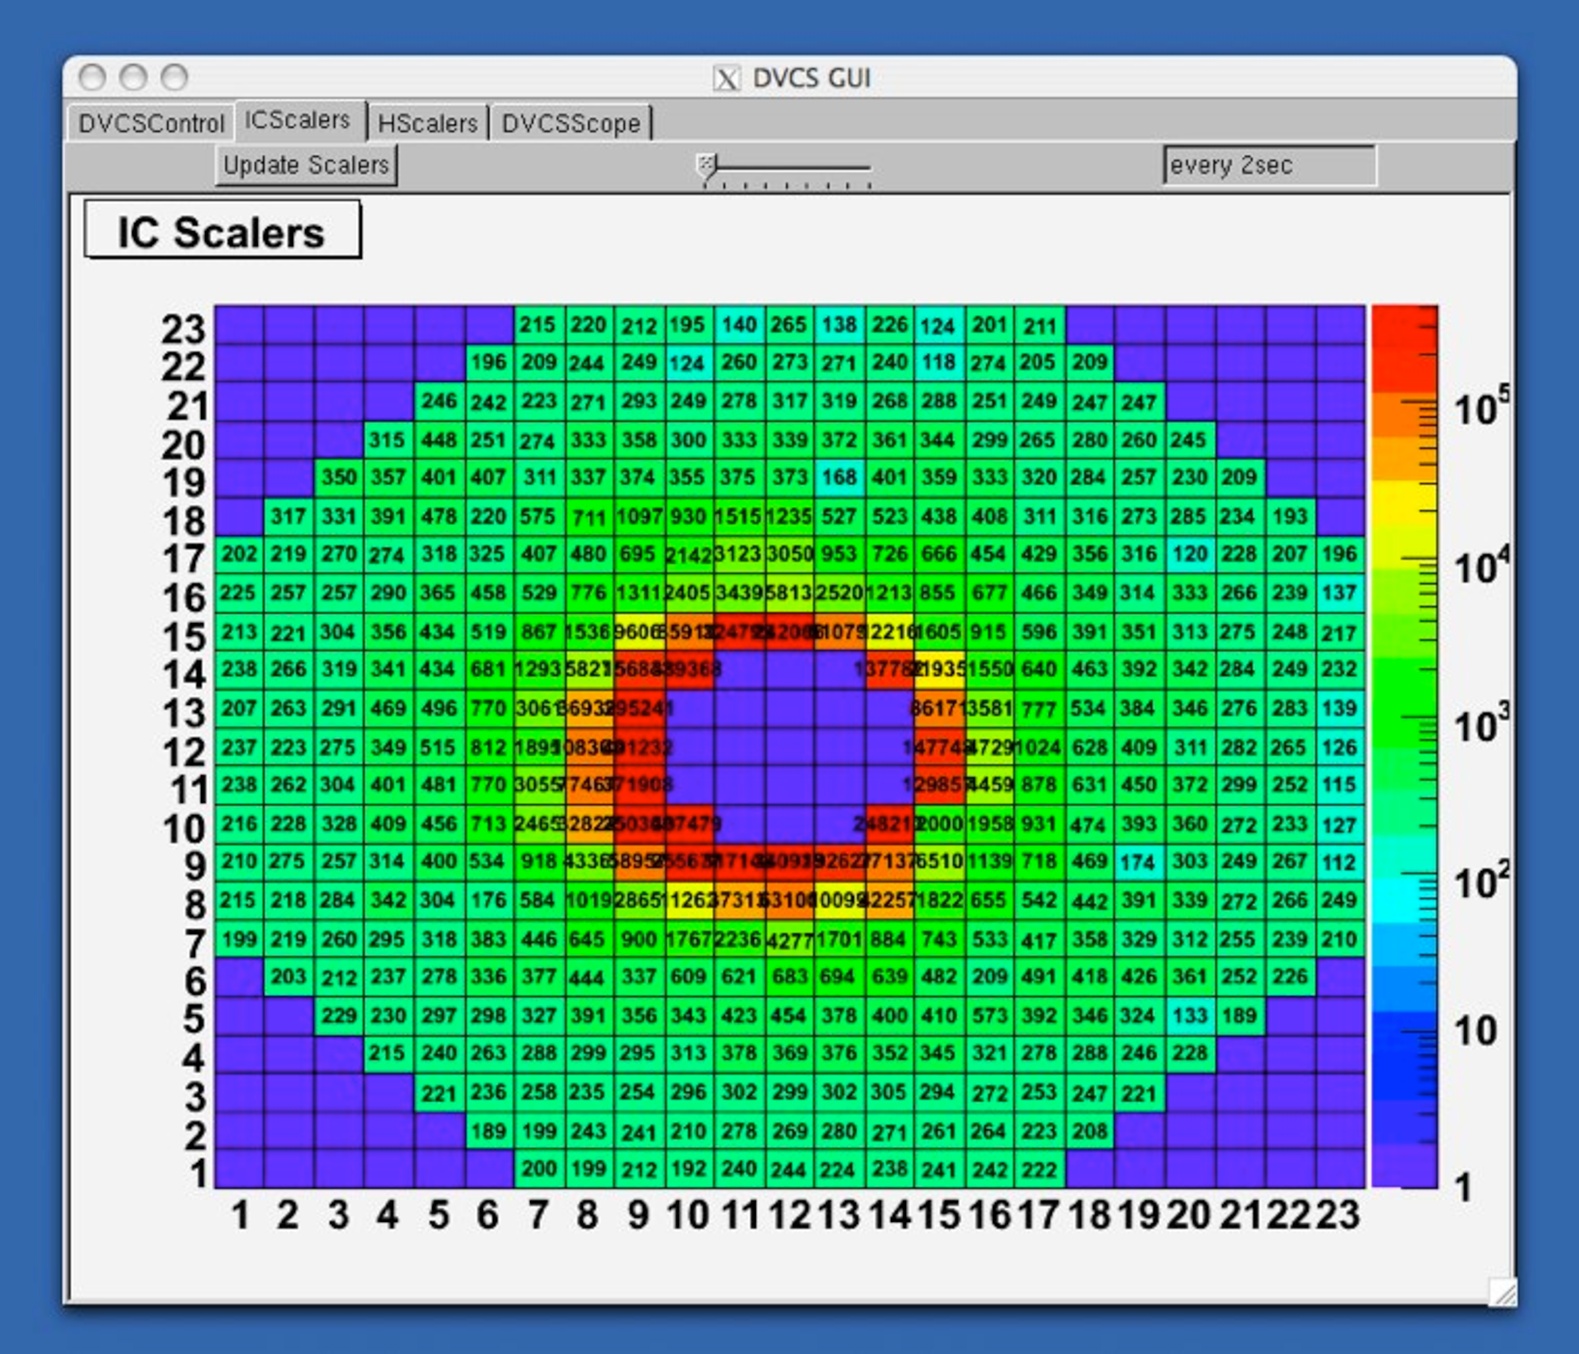
\includegraphics[scale=0.6]{daq_trigger/figures/dvcs_beam}
\caption{\small{Scalers (example from the previous version of the calorimeter).}}
\label{fig:dvcs_beam}
\end{figure}
Diagnostic scope permits to analyze on-line  the trigger logic. The goal to have  the Two-Dimensional Analyzer
 is to provide a remote debug interface to identify bad channels, verify cluster finding algorithms and check timing.
 The details of this analyzer are as following:
 
\begin{itemize}
\item Logic analyzer runs in parallel, non-intrusive, to the calorimeter trigger
\item Can setup trigger on any ECal pixel arrangement and/or cluster count
\item Can move forward/backward in time by ~250 ns to see timing details
\item Will be customize for HPS geometry and hardware
\end{itemize}

The example of the 2D analyzer is presented in Fig.~\ref{fig:dvcs_2_cluster}. Two clusters are displayed
in the picture. The red color displays the hits in the calorimeter and  the center of clusters is displayed in yellow.

In addition to the scalers, the distributions on individual ADC channel pulse energy will be provided.
The cluster hits positions and energy from SSP processor will be histogrammed as well. Two histograms (accepted and rejected) will be provided for each trigger cut used in the trigger logic.



\begin{figure}[t]
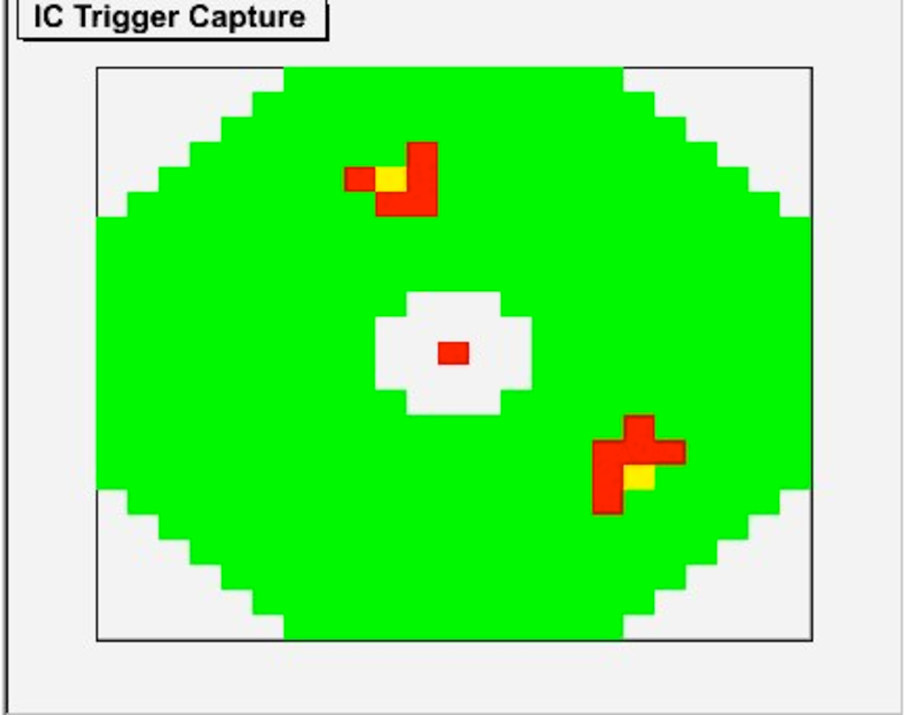
\includegraphics[scale=0.8]{daq_trigger/figures/dvcs_2_cluster}
\caption{\small{Diagnostic scope (example with two clusters found from the previous version of the calorimeter). Green - no hits, red - tower with hit, yellow - cluster found.}}
\label{fig:dvcs_2_cluster}
\end{figure}


%\subsubsection{Muon Trigger}

\subsubsection{Muon Trigger}

A muon detector composed of a four iron absorbers  and four double-layer scintillator planes, positioned after each absorber. Similar to the Ecal, the muon detector will consist of two halves, one above and one below the beam.
GEANT4 simulations have been used to study the trigger rates in the muon system due to background hits. It is expected that the true di-muon rate will be quite small compared to the ECal trigger rate and should not cause problem for the DAQ. 
A total of 144 readout channels are needed (9x16 channels multi-anode PMTs). Signals from each channel will be sent to a TDC and to a FADC. The FADC information will be used to construct the muon trigger. The TDC information together with information from FADC will be used in offline analysis to measure the hit position along the strip.

Selecting coincidence hits with MIP energy deposition in at least three layers of the scintillation hodoscope will identify muons. 
The muon trigger logic has to find one track in the top part of the detector in coincidence with another track in the bottom part of the detector. The track finding algorithm can be easily realized in the FPGA logic of the muon Crate Trigger processor.

